\chapter{Analisi dello schematico}

I principali componenti utilizzati per la realizzazione del progetto
sono:

\begin{itemize}
\item
  \begin{quote}
  microcontrollore \emph{RP2040};
  \end{quote}
\item
  \begin{quote}
  memoria flash \emph{QSPI} \emph{W25Q16JV};
  \end{quote}
\item
  \begin{quote}
  regolatore di tensione \emph{TPS563201};
  \end{quote}
\item
  \begin{quote}
  \emph{GPS PAM7Q};
  \end{quote}
\item
  \begin{quote}
  magnetometro \emph{HMC5883L};
  \end{quote}
\item
  \begin{quote}
  accelerometro e giroscopio \emph{MPU6050};
  \end{quote}
\item
  \begin{quote}
  2 motori stepper unipolari con riduttore \emph{28BYJ (ADAFRUIT 918)};
  \end{quote}
\item
  \begin{quote}
  circuiti di misura tensione e corrente;
  \end{quote}
\item
  \begin{quote}
  display \emph{OLED} 128x64;
  \end{quote}
\item
  \begin{quote}
  USB type B-mini;
  \end{quote}
\item
  \begin{quote}
  buzzer;
  \end{quote}
\item
  \begin{quote}
  led \emph{RGB 1210}.
  \end{quote}
\end{itemize}

Per una maggior chiarezza abbiamo deciso di dividere lo schematico in
più fogli, ognuno con una funzione ben precisa:

\begin{itemize}
\item
  \begin{quote}
  \textbf{Control}: \emph{MCU}, \emph{Flash}, Oscillatore al quarzo,
  pulsanti ecc..
  \end{quote}
\item
  \begin{quote}
  \textbf{Power}: Regolatore di tensione, \emph{USB}
  \end{quote}
\item
  \begin{quote}
  \textbf{Peripherals}: GPS, Magnetometro, Accelerometro, \emph{OLED},
  Buzzer, Led \emph{RGB}
  \end{quote}
\item
  \begin{quote}
  \textbf{Panel} \textbf{sensing}: Current sensing, Voltage Sensing
  \end{quote}
\item
  \begin{quote}
  \textbf{Actuation}: Stepper Driver
  \end{quote}
\end{itemize}

\begin{center}
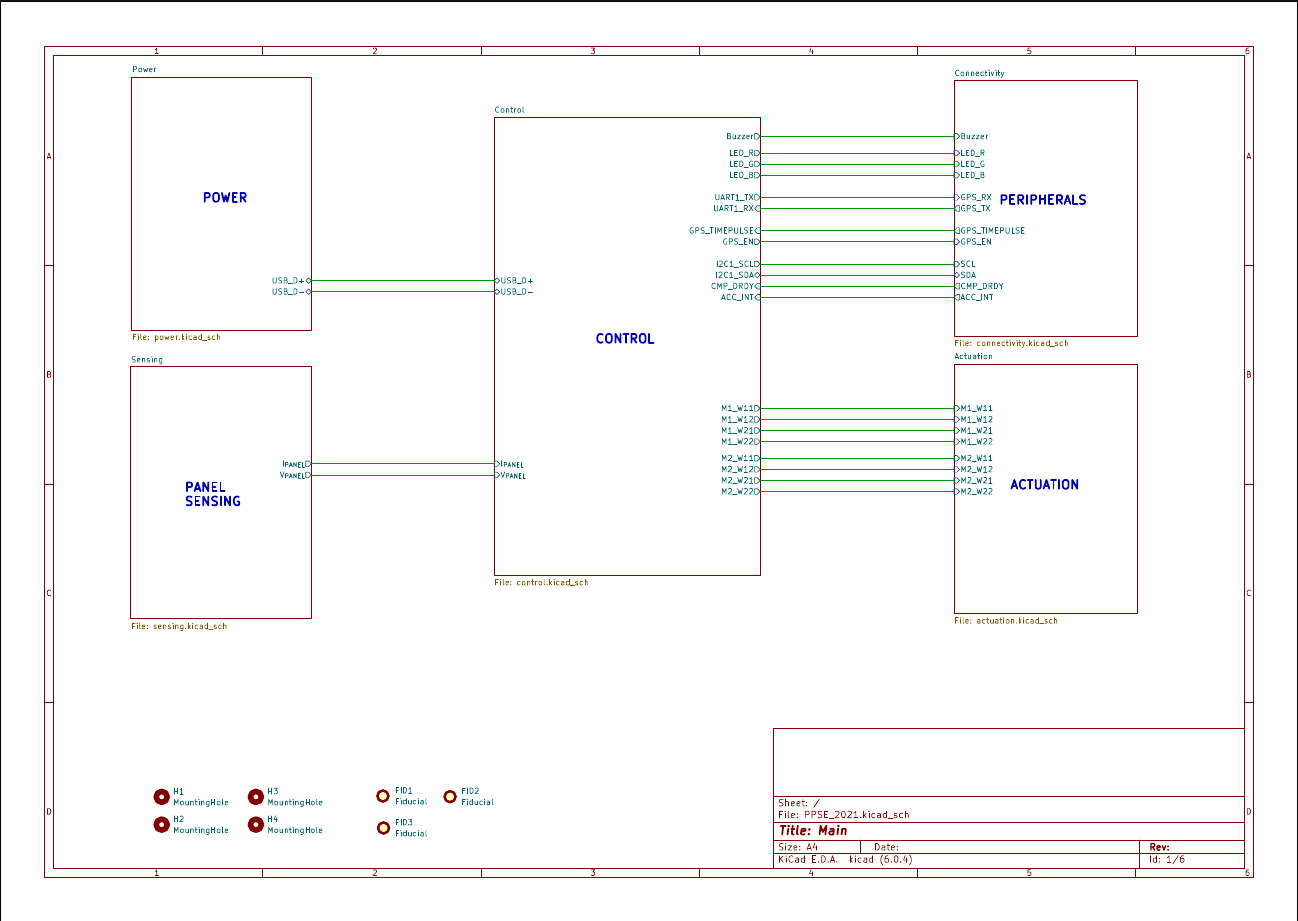
\includegraphics[width=6.5in,height=4.48in]{figures/image32.png}
\captionsetup{type=figure}
\captionof{figure}{Foglio "Main" SALMO}
\end{center}

\hypertarget{control}{%
\section{Control}\label{control}}

Il foglio ``\emph{Control}'' include i componenti adibiti al controllo
della scheda, quali:

\begin{itemize}
\item
  \begin{quote}
  microcontrollore \emph{RP2040};
  \end{quote}
\item
  \begin{quote}
  memoria flash SPI \emph{W25Q16JV};
  \end{quote}
\item
  \begin{quote}
  cristallo al quarzo a 12 \emph{MHz};
  \end{quote}
\item
  \begin{quote}
  pulsanti di reset, boot, home e tracking enable;
  \end{quote}
\item
  \begin{quote}
  connettori di debug ed espansione.
  \end{quote}
\end{itemize}

\begin{center}
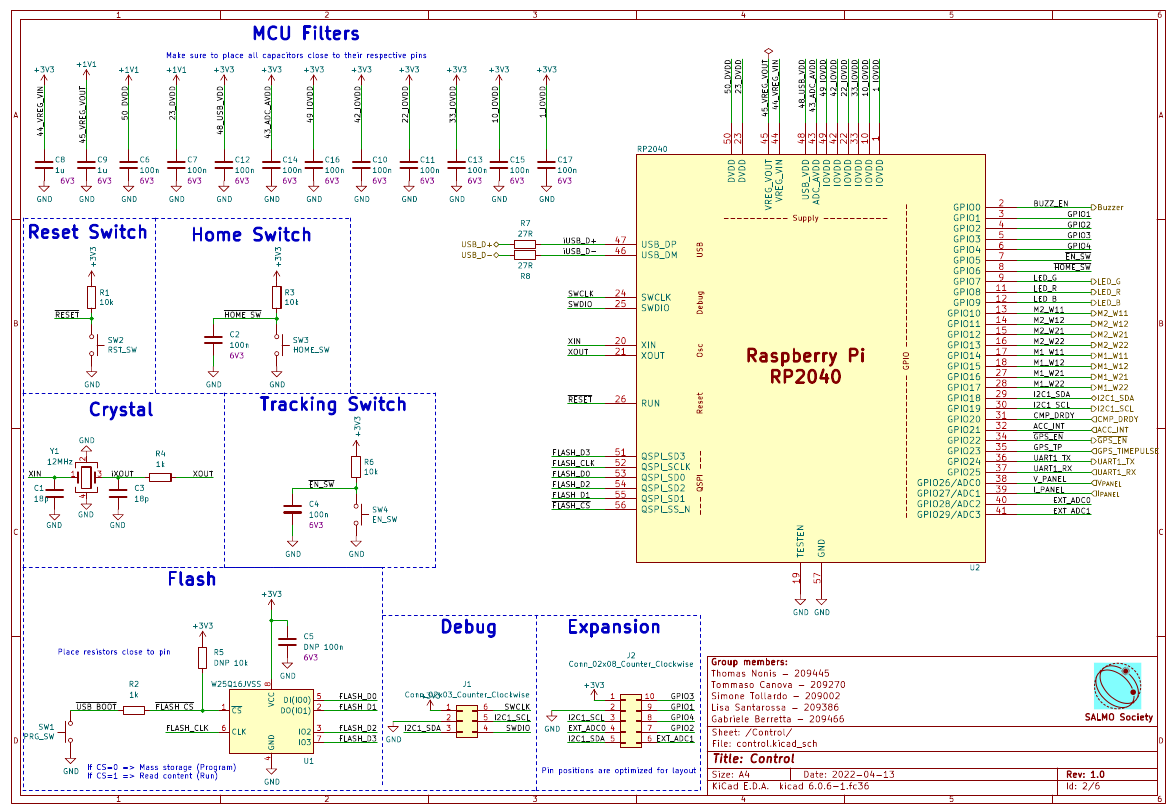
\includegraphics[width=6.5in,height=4.48611in]{figures/image40.png}
\captionsetup{type=figure}
\captionof{figure}{Foglio "Control" SALMO}
\end{center}

\hypertarget{microcontrollore-rp-2040}{%
\subsubsection{\texorpdfstring{\hfill\break
Microcontrollore: RP
2040}{ Microcontrollore: RP 2040}}\label{microcontrollore-rp-2040}}

La scheda si avvale dell'ormai celeberrimo \emph{MCU} di Raspberry Pi Ltd: \emph{RP2040}.

Caratteristiche principali:

\begin{itemize}
\item
  \begin{quote}
  133 \emph{MHz} dual core 32 bit ARM Cortex-M0+;
  \end{quote}
\item
  \begin{quote}
  264 \emph{KB} SRAM;
  \end{quote}
\item
  \begin{quote}
  Nessuna memoria flash interna;
  \end{quote}
\item
  \begin{quote}
  Controller bus \emph{QSPI}, che supporta fino a 16 MB di memoria flash
  esterna;
  \end{quote}
\item
  \begin{quote}
  Controllore \emph{DMA};
  \end{quote}
\item
  \begin{quote}
  Crossbar \emph{AHB} (Advanced High-performance Bus);
  \end{quote}
\item
  \begin{quote}
  Regolatore \emph{LDO} programmabile per generare la tensione del core
  integrato;
  \end{quote}
\item
  \begin{quote}
  2 \emph{PLL} su chip per generare clock USB e core;
  \end{quote}
\item
  \begin{quote}
  30 pin \emph{GPIO}, di cui 4 utilizzabili opzionalmente come ingressi
  analogici.
  \end{quote}
\end{itemize}

Periferiche:

\begin{itemize}
\item
  \begin{quote}
  2 \emph{UART};
  \end{quote}
\item
  \begin{quote}
  2 controller \emph{SPI};
  \end{quote}
\item
  \begin{quote}
  2 controller \emph{I²C};
  \end{quote}
\item
  \begin{quote}
  16 canali \emph{PWM};
  \end{quote}
\item
  \begin{quote}
  Controller USB 1.1 e \emph{PHY}, con supporto per host e dispositivo;
  \end{quote}
\item
  \begin{quote}
  8 macchine a stati di input-output (\emph{PIO}) programmate.
  \end{quote}
\end{itemize}

Il microcontrollore ha il compito di gestire le periferiche. In
particolare:

\begin{itemize}
\item
  \begin{quote}
  genera il segnale di rotazione dei motori quando previsto
  dall'algoritmo implementato (\emph{GPIO} da 10 a 17);
  \end{quote}
\item
  \begin{quote}
  comunica con il GPS tramite interfaccia UART (\emph{GPIO} 24 e 25);
  \end{quote}
\item
  \begin{quote}
  comunica con il magnetometro, con l'accelerometro e con il display
  OLED mediante interfaccia I2C (\emph{GPIO} 18 \emph{SDA}, \emph{GPIO}
  19 \emph{SCL});
  \end{quote}
\item
  \begin{quote}
  effettua le misure di corrente e di tensione del pannello (\emph{GPIO}
  26 e 27);
  \end{quote}
\item
  \begin{quote}
  gestisce il buzzer (\emph{GPIO} 0) ed un led \emph{RGB} (\emph{GPIO}
  7, 8, 9);
  \end{quote}
\item
  \begin{quote}
  comunica con la memoria \emph{flash} (pin da 51 a 56);
  \end{quote}
\item
  \begin{quote}
  gestisce l'interfaccia \emph{USB} (pin 46 e 47).
  \end{quote}
\end{itemize}

\begin{center}
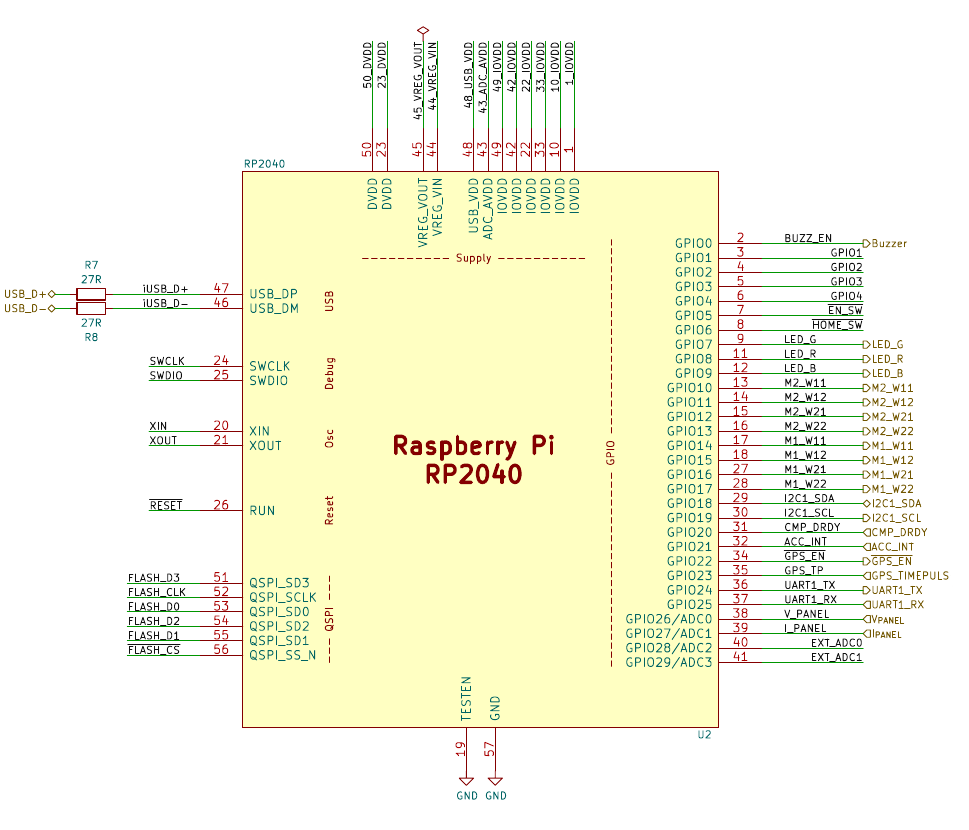
\includegraphics[width=6.5in,height=5.56944in]{figures/image54.png}
\captionsetup{type=figure}
\captionof{figure}{Schema pin microcontrollore RP2040\newline}
\end{center}

Per ridurre il rumore ad alta frequenza presente sulla linea di
alimentazione abbiamo previsto dei condensatori di filtro per
cortocircuitare a massa la componente alternata (andranno poi
posizionati il più vicino possibile ai pin del MCU).

\begin{center}
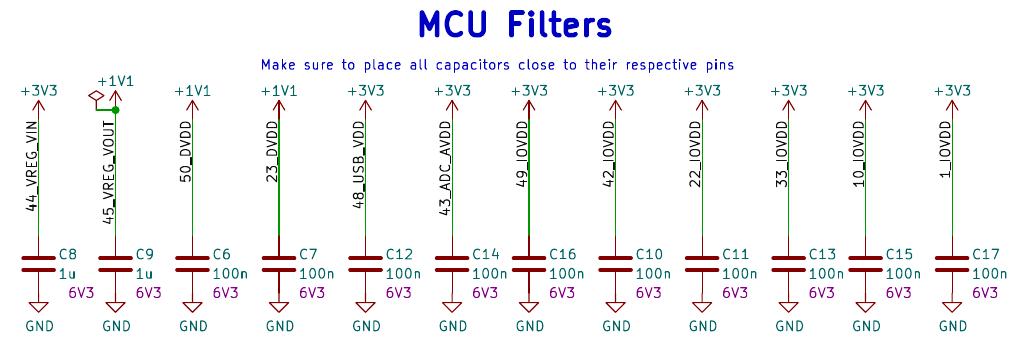
\includegraphics[width=6.33776in,height=2.22396in]{figures/image23.png}
\captionsetup{type=figure}
\captionof{figure}{Condensatori di bypass MCU}
\end{center}

\hypertarget{pulsanti}{%
\subsubsection{\texorpdfstring{\hfill\break
Pulsanti}{ Pulsanti}}\label{pulsanti}}

Per il progetto \emph{SALMO} abbiamo previsto quattro switch:

\begin{itemize}
\item
  \begin{quote}
  Un pulsante di reset (\emph{SW2}) per poter resettare il
  microcontrollore;
  \end{quote}
\item
  \begin{quote}
  Un pulsante per portare il microcontrollore in modalità
  \emph{bootloader (SW1)}, in modo tale da poter ``flashare'' il
  programma via USB.
  \end{quote}
\item
  \begin{quote}
  Un pulsante (\emph{SW3}), denominato "Home", che permette di portare
  il sistema di puntamento del pannello solare ad una posizione
  predefinita (0° Nord, 45° Elevazione);
  \end{quote}
\item
  \begin{quote}
  Un pulsante (\emph{SW4}), denominato ``Tracking Enable'', che permette
  di far partire il sistema di puntamento del pannello;
  \end{quote}
\end{itemize}

\begin{center}
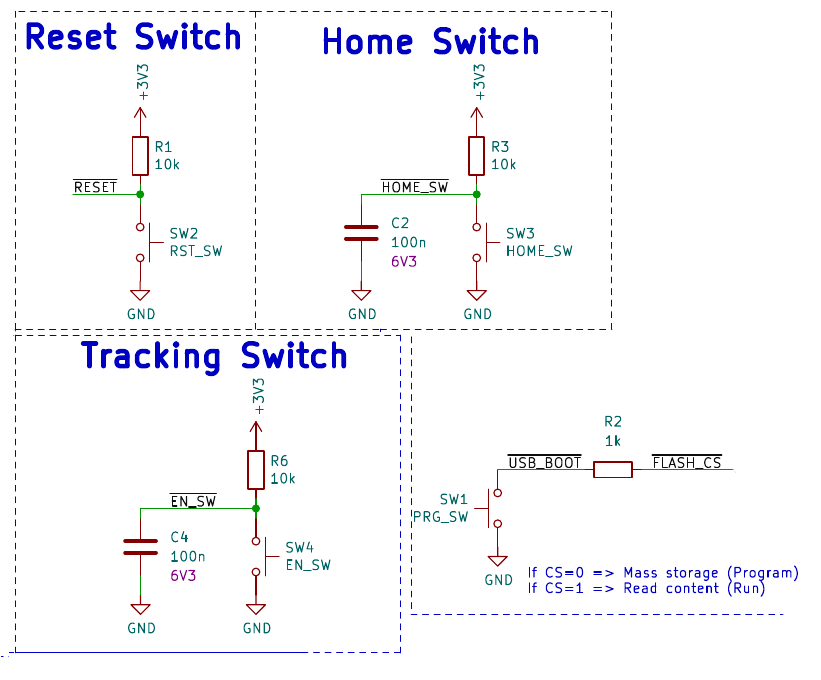
\includegraphics[scale=0.5]{figures/image16.png}
\captionsetup{type=figure}
\captionof{figure}{Pulsanti SALMO}
\end{center}

Per ogni pulsante abbiamo previsto un resistore di pull-up da 10kΩ, che
nel caso del pulsante di programmazione è contrassegnato come \emph{DNP}
(Do Not Place), poiché la memoria fornisce un \emph{pull-up} interno che
lo rende non necessario.

Per i pulsanti di \emph{reset} e programmazione non abbiamo previsto
alcun filtro di debouncing come consigliato dai relativi datasheet,
mentre per i restanti abbiamo aggiunto un condensatore da \emph{100nF}
per introdurre una costante di tempo di \emph{1ms}.

La resistenza R2 in serie al pulsante di programmazione è stata inserita
seguendo i consigli del manuale di sviluppo hardware del RP2040
(probabilmente il pin $\overline{\rm {CS}}$ della flash non ha una
resistenza di limitazione interna).

I pulsanti scelti sono dei generici \emph{tactile switch} da 6mm a
tecnologia TH .

\hypertarget{quarzo}{%
\subsubsection{Quarzo}\label{quarzo}}

Per generare il segnale di clock del microcontrollore abbiamo
selezionato un quarzo da 12 \emph{MHz}. In particolare abbiamo
utilizzato un quarzo a 4 pin con package \emph{3225}, essendo questo uno
dei constraint imposti dal professore ad inizio progetto. Per il
dimensionamento del resistore in serie e dei condensatori abbiamo
seguito le linee guida del manuale di sviluppo hardware del RP2040.

\(C_{1} = C_{2} = 2 \cdot (C_{L} - C_{\text{Parassita}})\)
, dove \(C_{L}\) è la capacità di load ottimale del quarzo.

Ipotizzando quindi una capacità parassita pari a 5pF ed una capacità di
load di 14pF otteniamo \(C_{1} = C_{2} =18pF\).

\begin{center}
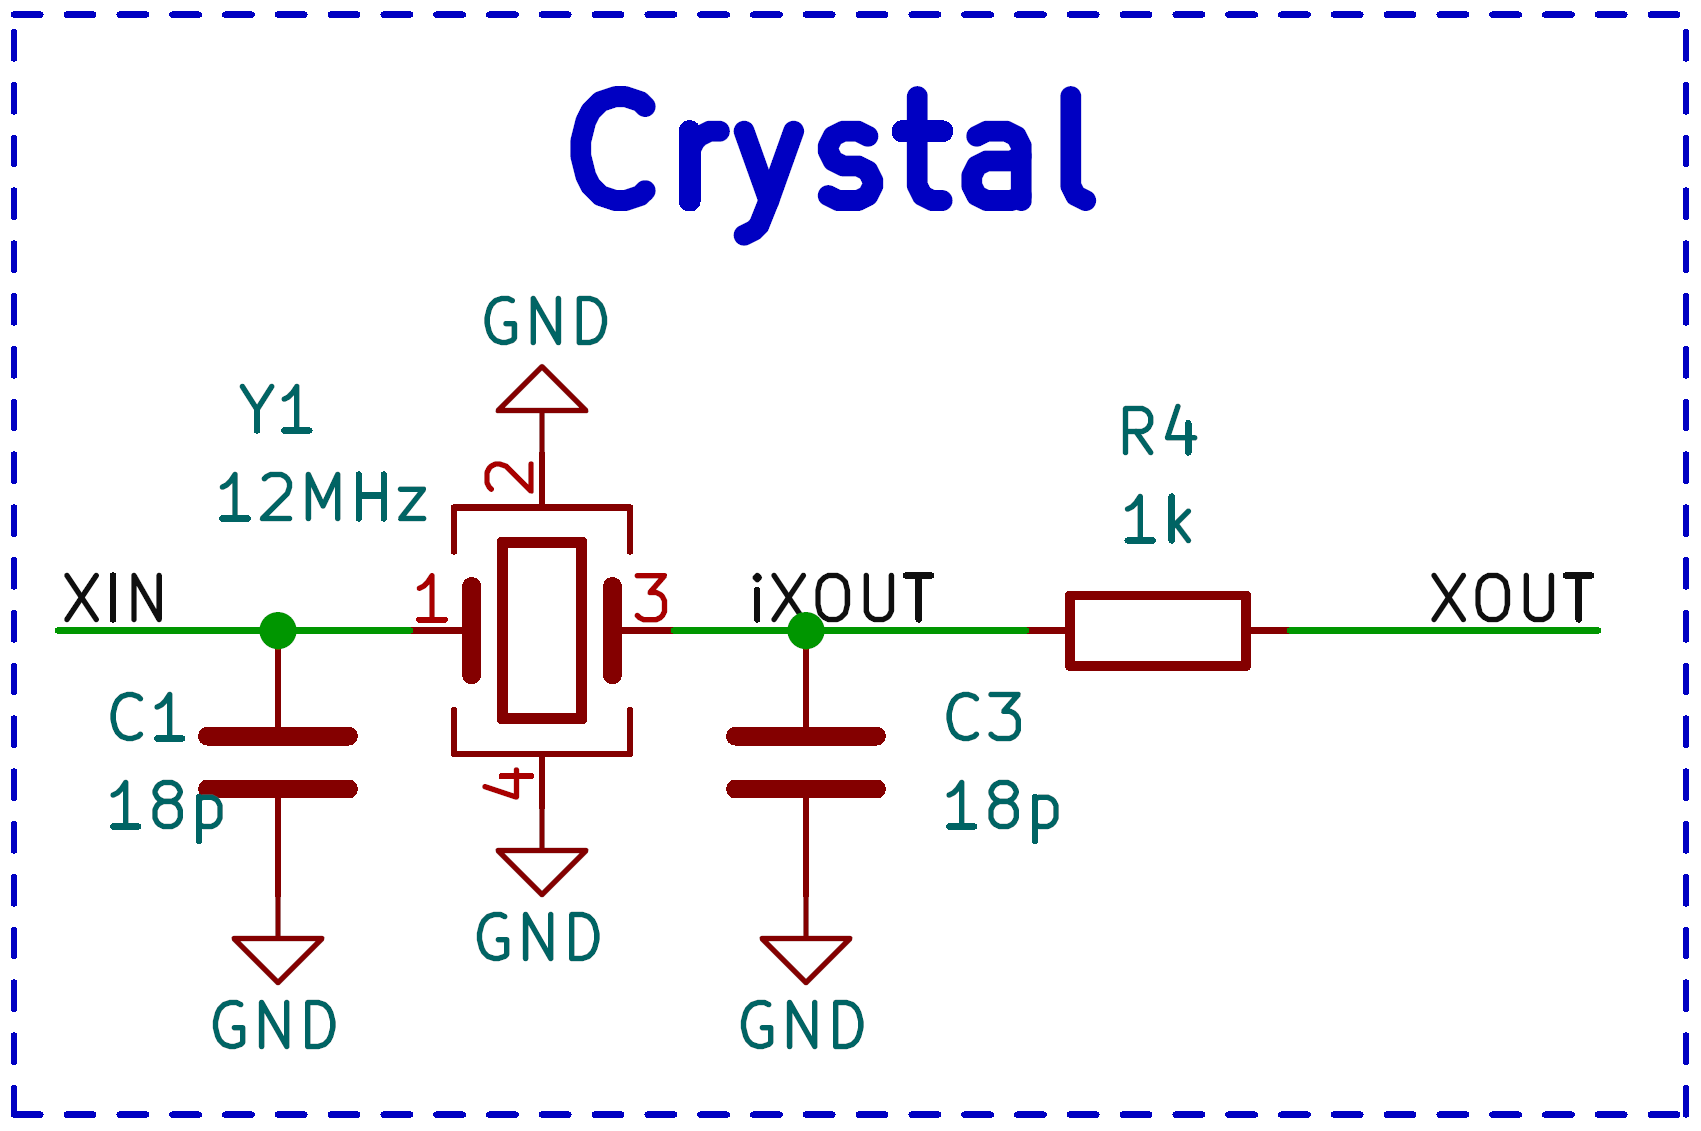
\includegraphics[scale=0.8]{figures/image76.png}
\captionsetup{type=figure}
\captionof{figure}{Circuito del cristallo di quarzo di SALMO\newline}
\end{center}

La capacità di carico è particolarmente importante perché, essendo la
capacità totale vista dai due pin del cristallo XIN e XOUT, può portare
il cristallo ad oscillare in un punto specifico tra la sua frequenza
minima e massima. Cambiando la capacità del carico si otterrà quindi una
diversa frequenza di oscillazione. Ecco perché il produttore di
cristalli fornisce la frequenza del cristallo a una capacità di carico
specifica, che in questo caso è di 14pF.

\begin{center}
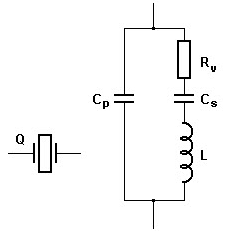
\includegraphics[width=2.38542in,height=2.45833in]{figures/image28.png}
\captionsetup{type=figure}
\captionof{figure}{Modello RLC di un cristallo al quarzo in risonanza parallelo}
\end{center}

\hypertarget{memoria-flash}{%
\subsubsection{\texorpdfstring{\hfill\break
Memoria flash}{ Memoria flash}}\label{memoria-flash}}

Nella memoria flash viene salvato il firmware compilato in formato
\emph{.uf2}, il quale all'accensione verrà eseguito dal bootloader. La
memoria flash utilizzata è la \emph{W25Q16JV}, e viene interfacciata
mediante protocollo QSPI (Quad-SPI). Questo tipo di comunicazione è
particolarmente diffuso nel ramo delle comunicazioni con memorie flash,
come nel caso presente sulla scheda. Rispetto allo standard SPI, sono
presenti 4 linee di dato bidirezionali, rispettivamente \emph{I0, I1,
I2, I3} (che vanno dunque a sostituire \emph{MISO} e \emph{MOSI}), che
permettono un trasferimento dati più veloci dalle 4 alle 6 volte
rispetto normale SPI (secondo il datasheet).

\begin{center}
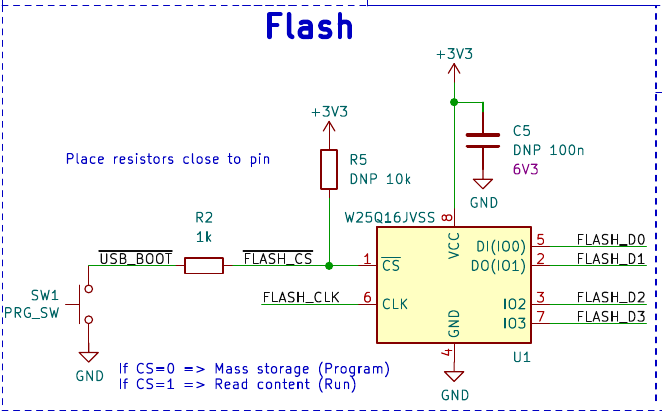
\includegraphics[width=6.5in,height=4.05556in]{figures/image49.png}
\captionsetup{type=figure}
\captionof{figure}{Circuito flash SALMO}
\end{center}

Il pin $\overline{\rm {CS}}$ permette di abilitare o
disabilitare la comunicazione \emph{QSPI}, quando $\overline{\rm {CS}}$=1 i pin di
comunicazione rimangono ad alta impedenza, mentre quando $\overline{\rm {CS}}$=0 è
possibile interfacciarsi con la memoria per memorizzare il programma. È
inoltre presente un condensatore da 100nF per filtrare rumore ad alta
frequenza in alimentazione.

\hypertarget{debug-ed-espansione}{%
\subsubsection{\texorpdfstring{\hfill\break
Debug ed espansione}{ Debug ed espansione}}\label{debug-ed-espansione}}

\begin{center}
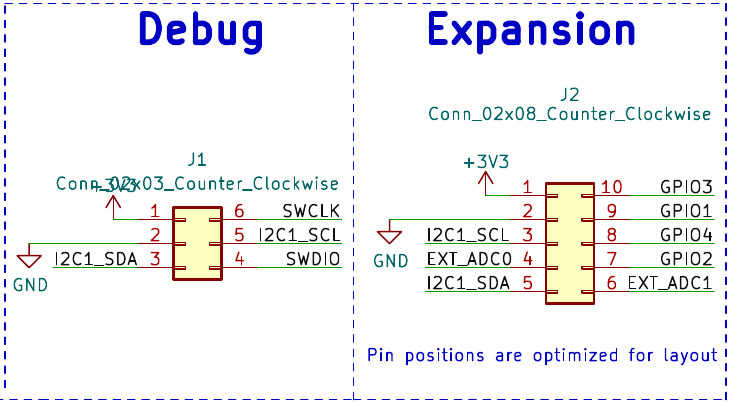
\includegraphics[scale=0.8]{figures/image90.png}
\captionsetup{type=figure}
\captionof{figure}{Connettori Debug ed Expansion SALMO\newline}
\end{center}

Per permettere al microcontrollore di comunicare con eventuali unità
esterne, sulla scheda abbiamo inserito un connettore a 10 pin con le
linee \emph{I2C}, i due canali non utilizzati del convertitore analogico
digitale ed i rimanenti \emph{GPIO} non utilizzati.\\
Abbiamo previsto anche un connettore per il debug con interfaccia SWD
(\emph{Serial Wire Debug}), alimentazione per il microcontrollore e bus
\emph{I2C}. Per il debug è necessario utilizzare un altro \emph{RP2040},
potrebbe essere particolarmente conveniente utilizzare un Pi Pico come
debugger, viste le due dimensioni. Basta collegare le linee di SWData e
SWClock tra loro e la relativa alimentazione necessaria al debugger,
dopodichè si può flashare quest'ultimo con \emph{picoprobe.uf2}
(programma situato nella cartella degli esempi offerti per RP2040,
vedesi capitolo
\protect\hyperlink{_w8kvxnysumpc}{\underline{Firmware}}), per poi
interfacciarsi via usb utilizzando GDB ed OpenOCD.

\begin{center}
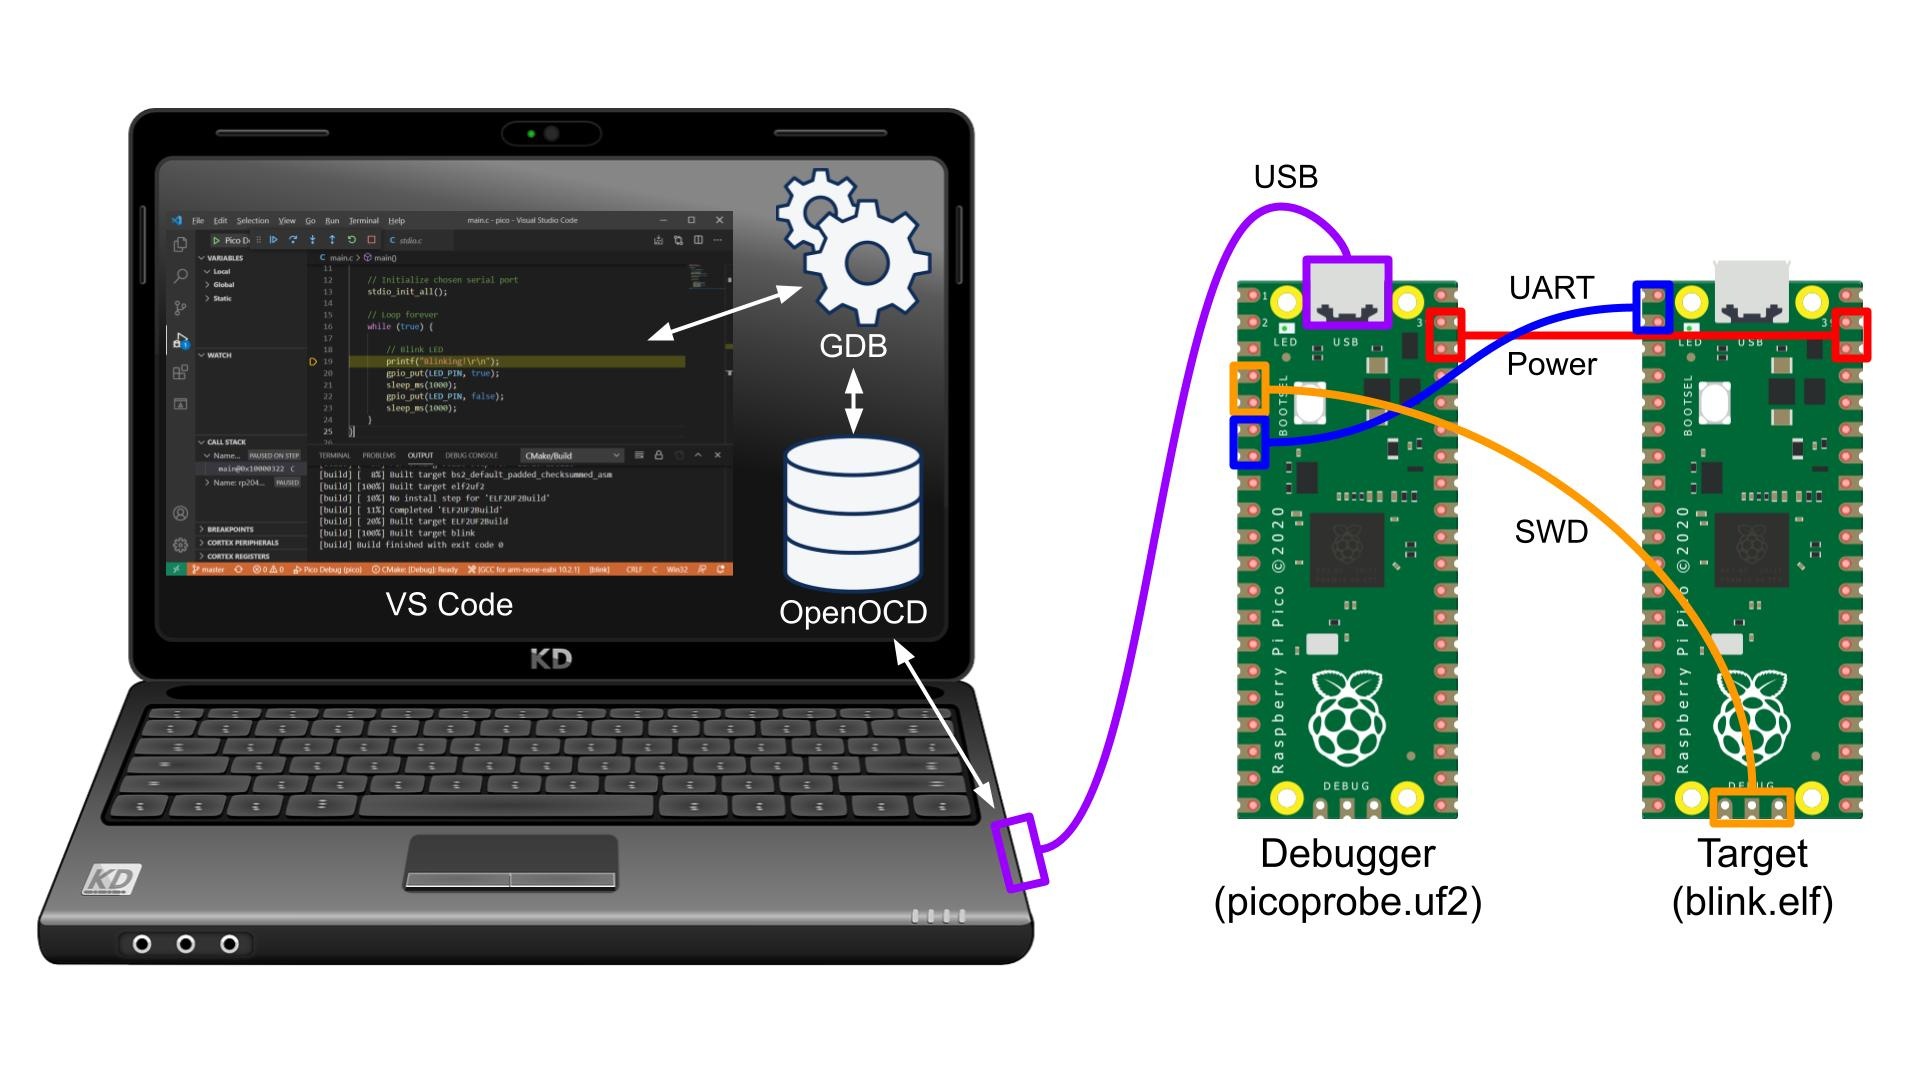
\includegraphics[width=6.5in,height=3.65278in]{figures/image18.png}
\captionsetup{type=figure}
\captionof{figure}{Immagine illustrativa del debug di un Pi Pico mediante un altro Pi Pico}
\end{center}

\hypertarget{power}{%
\section{Power}\label{power}}

\begin{center}
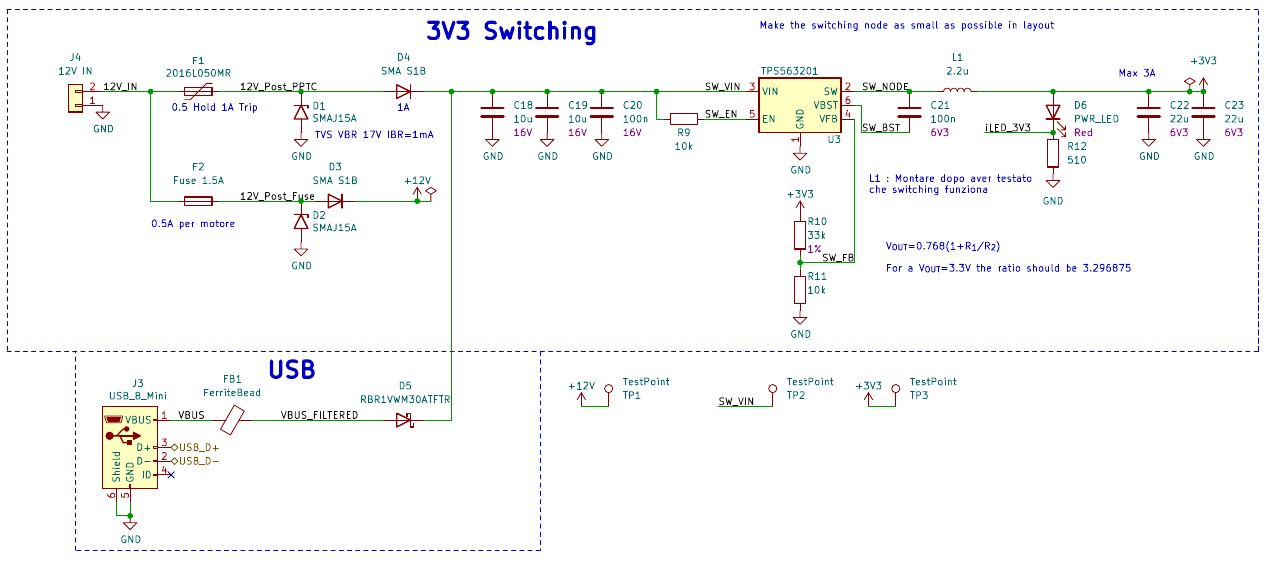
\includegraphics[width=6.5in,height=3.65278in]{figures/image65.png}
\captionsetup{type=figure}
\captionof{figure}{Foglio "Power" SALMO\newline}
\end{center}

L'alimentazione principale della scheda (+12V) proviene dal connettore
J4 e verrà successivamente ``divisa'' in due rami: regolatore di
tensione e alimentazione dei motori.

\begin{center}
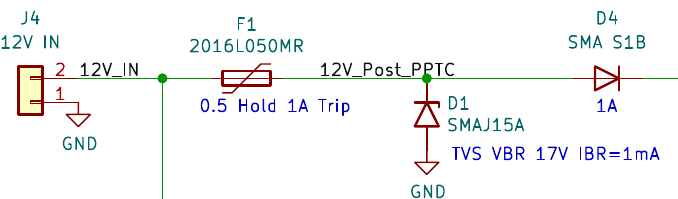
\includegraphics[scale=0.8]{figures/image80.png}
\captionsetup{type=figure}
\captionof{figure}{Ramo regolatore di tensione\newline}
\end{center}

\begin{center}
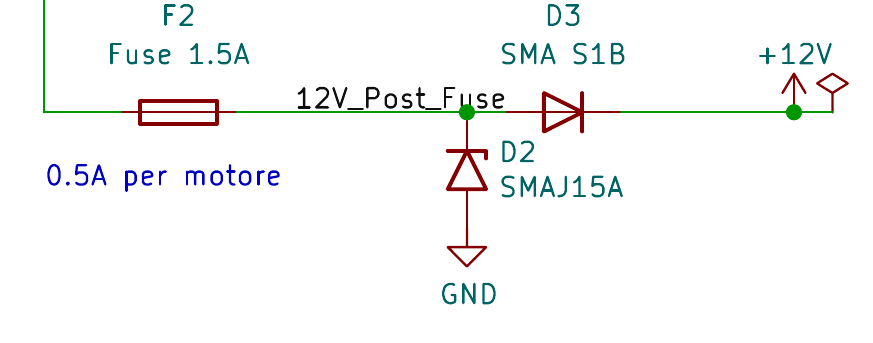
\includegraphics[scale=0.6]{figures/image64.png}
\captionsetup{type=figure}
\captionof{figure}{Ramo alimentazione motori\newline}
\end{center}

La scheda può essere alimentata anche tramite un connettore \emph{USB}
di tipo B-mini (il pin \emph{ID} è stato lasciato flottante non dovendo
utilizzare la funzione \emph{USB OTG}, fissando il dispositivo come
device), ovviamente non potendo alimentare motori e led \emph{RGB}.\\
Per evitare i rumori ad alta frequenza la tensione di bus viene filtrata
tramite una \emph{ferrite bead}, la quale sfrutta le medesime proprietà
dell'induttore, esercitando una resistenza 120 Ω a 100 MHz.

È necessaria inoltre la presenza del diodo schottky \emph{D5} per
evitare che i 12V possano propagarsi fino alla rail dei 5V dell'USB.

\begin{center}
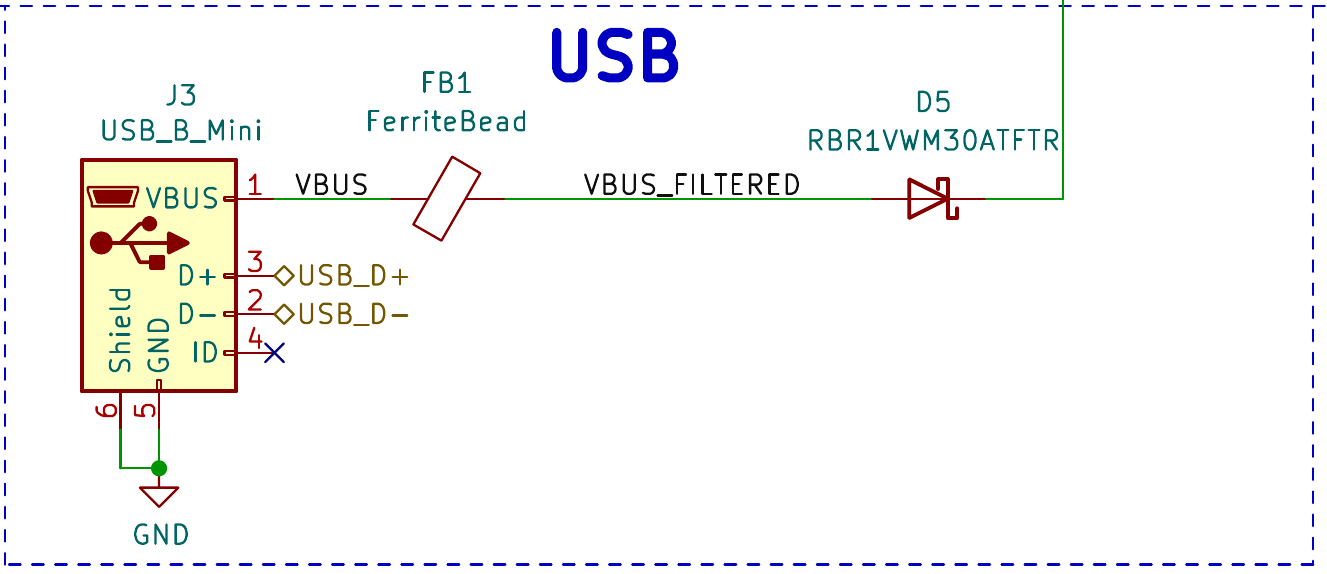
\includegraphics[width=6.5in,height=2.80556in]{figures/image60.png}
\captionsetup{type=figure}
\captionof{figure}{Alimentazione via USB\newline}
\end{center}

I diodi \emph{D4} e \emph{D5} sono imperativi e svolgono la funzione di
\emph{OR logico} per garantire in ogni caso l'alimentazione al
regolatore switching.

Il fusibile \emph{F2} serve per proteggere i driver dei motori ed i
motori stessi dalle sovracorrenti, mentre a protezione del
microcontrollore e delle periferiche è stato previsto il fusibile
resettabile \emph{F1}, un \emph{PPTC} (polymeric positive temperature
coefficient). Quest'ultimo è in grado di aumentare la sua resistenza
all'aumentare della temperatura, riducendo così il passaggio di corrente
nel ramo.\\
La corrente massima assorbita da ciascun motore è di circa 0.5 A, perciò
abbiamo scelto un fusibile da 1.5 A (lasciando qualche centinaio di mA
per il led \emph{RGB} e qualche altro per avere una minima
tolleranza).\\
Il diodo \emph{SMAJ15A} è invece un diodo TVS, cioè un dispositivo
\emph{p-n} studiato per assorbire correnti elevate di eventi transitori
elettrici.

Il regolatore di tensione utilizzato è un \emph{TPS563201}, con tensione
in ingresso minima di 4.5V e massima di 17V. Per poter avere in output
una tensione di 3.3V, il pin VFB del regolatore deve essere connesso tra
due resistenze di rapporto \(\frac{R10}{R11} = \ 3.3\) considerando che
la formula per dimensionare Vout, ottenuta dal datasheet, è
\(Vout = 0.768(1 + \frac{R10}{R11})\).\\
Al fine di segnalare la presenza dei 3.3V, abbiamo previsto un led rosso
con resistenza in serie da 510 Ω.

\begin{center}
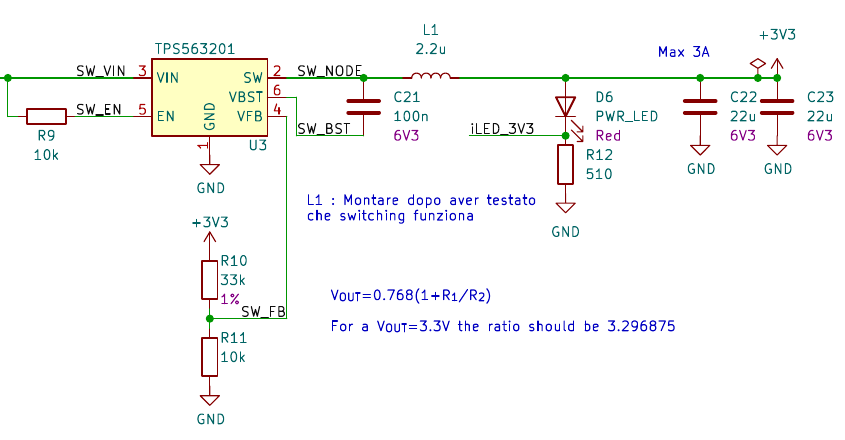
\includegraphics[scale=0.7]{figures/image57.png}
\captionsetup{type=figure}
\captionof{figure}{Circuito regolatore di tensione buck}
\end{center}

All'ingresso del regolatore di tensione abbiamo posto tre condensatori
(due da 10u e uno da 100n) con lo scopo di ridurre il ripple in uscita
dal regolatore switching. Si inseriscono 3 condensatori poiché, essendo
componenti reali e presentando di conseguenza una resistenza ed una
induttanza parassita, la loro combinazione darà luogo ad un condensatore
con caratteristiche migliori rispetto ad un condensatore di capacità
pari alla loro somma.

\begin{center}
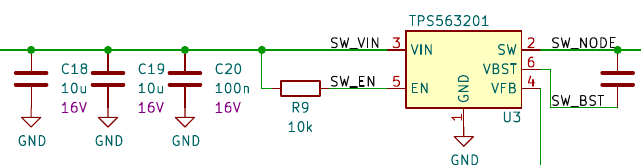
\includegraphics[scale=0.8]{figures/image71.png}
\captionsetup{type=figure}
\captionof{figure}{Condensatori in ingresso al regolatore di tensione\newline}
\end{center}

\begin{center}
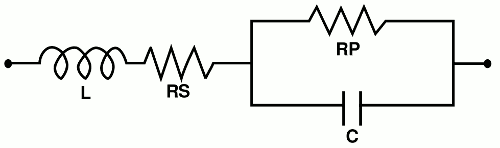
\includegraphics[scale=0.8]{figures/image37.png}
\captionsetup{type=figure}
\captionof{figure}{Modello RLC di un condensatore reale\newline}
\end{center}

Abbiamo infine previsto dei test point per il controllo delle varie
tensioni sul pannello.

\begin{center}
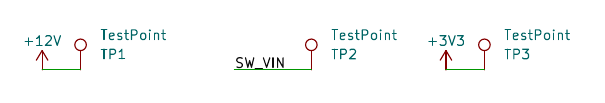
\includegraphics[scale=1]{figures/image78.png}
\captionsetup{type=figure}
\captionof{figure}{Testpoint per la misura delle tensioni di alimentazione}
\end{center}

\hypertarget{peripherals}{%
\section{Peripherals}\label{peripherals}}

\begin{center}
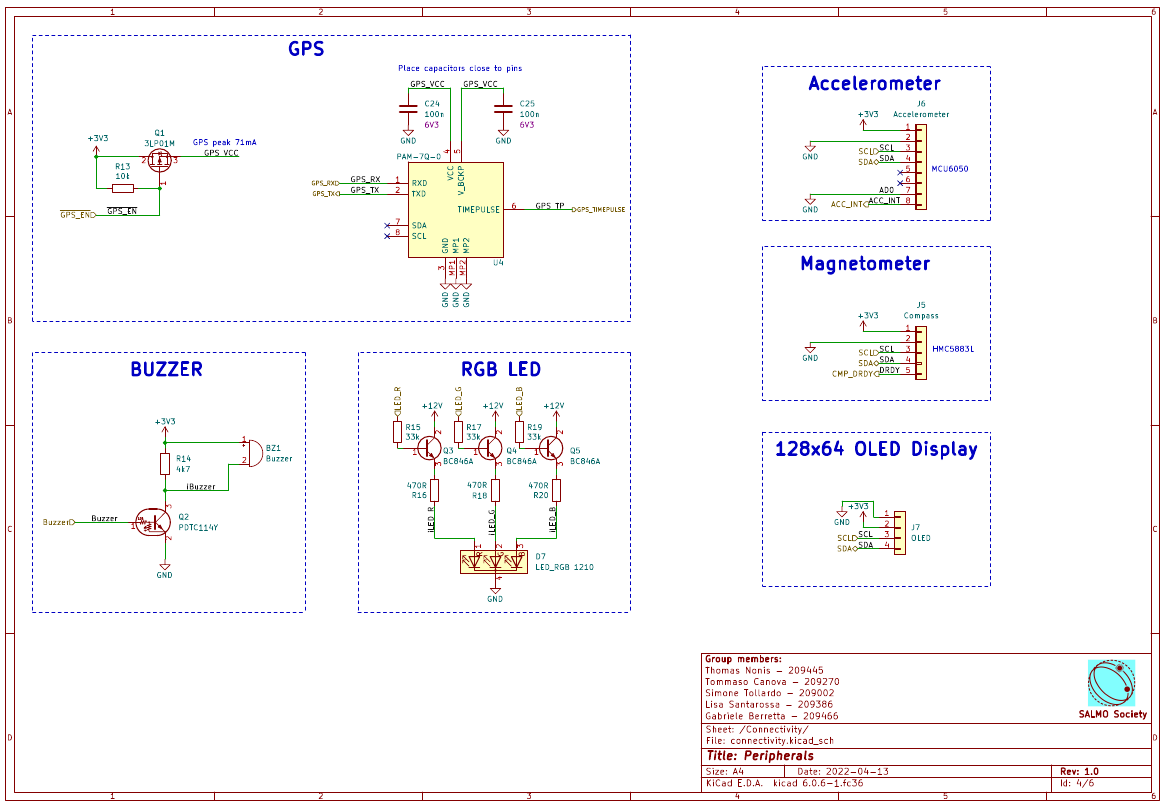
\includegraphics[width=6.5in,height=4.48611in]{figures/image15.png}
\captionsetup{type=figure}
\captionof{figure}{Foglio "Peripherals" SALMO}
\end{center}

\hypertarget{gps}{%
\subsubsection{\texorpdfstring{\hfill\break
\hfill\break
GPS }{  GPS }}\label{gps}}

Il dispositivo \emph{GPS} utilizzato è il \emph{U-BLOX PAM7Q}. Questo
componente serve per poter ottenere dai satelliti e la coordinate
geografiche del dispositivo \emph{SALMO}, in modo tale che il
microcontrollore possa calcolare la posizione del Sole rispetto al
pannello attraverso l'algoritmo di tracciamento e successivamente
stabilire il movimento dei motori.\\
Il dispositivo utilizza il protocollo standard \emph{NMEA} (ma può
essere configurato anche per utilizzare il protocollo proprietario
\emph{U-BLOX}) per comunicare attraverso la linea seriale.

\begin{center}
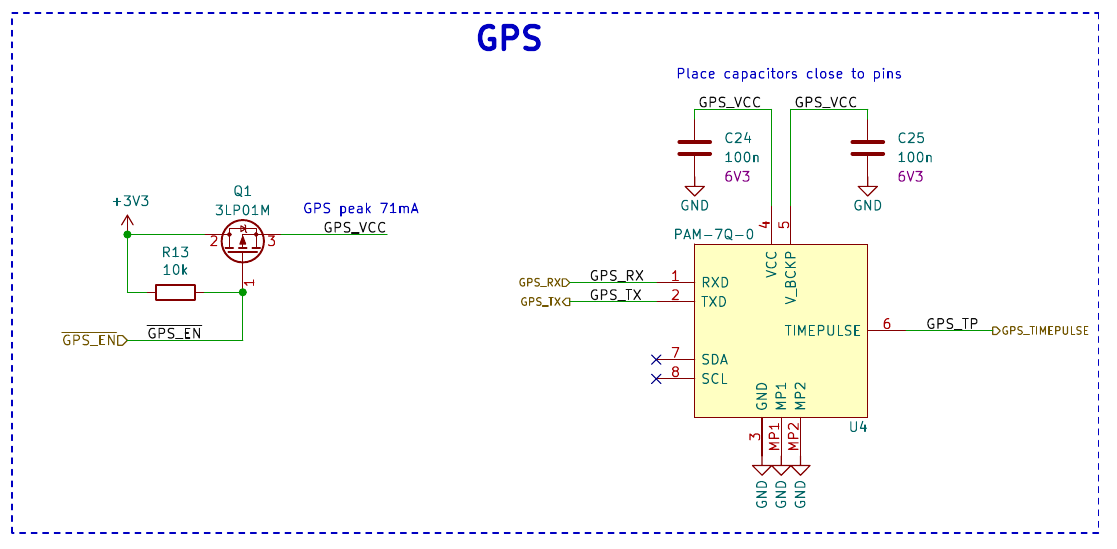
\includegraphics[width=6.5in,height=3.19444in]{figures/image26.png}
\captionsetup{type=figure}
\captionof{figure}{Circuito del GPS PAM7Q\newline}
\end{center}

Il dispositivo è alimentato a \emph{3V3} tramite i pin 4 e 5, si noti
che \emph{V\_BCKP} e \emph{VCC} sono entrambe connesse alla stessa
alimentazione, in quanto non è stata prevista una batteria tampone. Sono
presenti nuovamente i condensatori da 100nF tra \emph{GPS\_VCC} e ground
servono a bypassare il rumore ad alta frequenza verso massa.

L'alimentazione è interrotta da un transistor \emph{PMOS} (\emph{Q1}) e
viene abilitata solo quando il transistor viene polarizzato
correttamente, ovvero quando \textasciitilde(\emph{GPS\_EN}) si trova a
livello logico basso. La resistenza da 10kΩ tra gate e source del pmos
serve a mantenere il transistor in cut off quando il pin
\textasciitilde(\emph{GPS\_EN}) non è pilotato (floating).\\
I pin 1 e 2, cioè \emph{RXD} e \emph{TXD}, sono rispettivamente i pin di
ricezione e trasmissione per la comunicazione \emph{UART} (rispetto al
\emph{GPS}).\\
Il pin 6 è dedicato al time pulse, ovvero a generare un segnale
elettrico a 1 \emph{PPS} (pulse per second). Questa uscita può essere
utilizzata, ad esempio, per riattivare l'MCU da una modalità di
sospensione una volta al secondo per comunicare con esso. Il \emph{GPS}
\emph{PAM7Q} presenta anche un interfaccia seriale \emph{I2C} ma, dato
che per il progetto \emph{SALMO} abbiamo scelto un interfacciamento via
\emph{UART,} i pin 7 e 8 (\emph{SDA} e \emph{SCL}) sono stati lasciati
flottanti.\\
I mounting point \emph{MP1} e \emph{MP2} sono collegati a massa come
indicato da datasheet.

\begin{center}
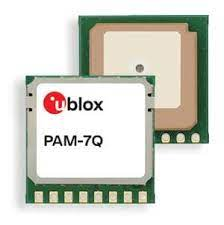
\includegraphics[scale=0.8]{figures/image30.jpg}
\captionsetup{type=figure}
\captionof{figure}{GPS U-Blox PAM7Q}
\end{center}

\hypertarget{magnetometro-ed-accelerometro}{%
\subsubsection{\texorpdfstring{\hfill\break
Magnetometro ed Accelerometro\\
}{ Magnetometro ed Accelerometro }}\label{magnetometro-ed-accelerometro}}

Al fine di poter gestire la posizione del pannello mediante controllo ad
anello chiuso abbiamo deciso di sfruttare due sensori: un magnetometro a
3 assi a 12 bit \emph{Honeywell} \emph{HMC5883L} ed un
accelerometro+giroscopio entrambi a 3 assi a 16 bit \emph{TDK}
\emph{MPU6050}, tutti e 2 con interfaccia \emph{I2C} a 400KHz massimi.\\
Questi, saranno posizionati \textbf{direttamente sul pannello} e
provvederanno a restituire all'algoritmo la posizione del pannello
rispetto ai due assi di movimento (Azimuth ed Elevazione).

Tuttavia, non avendo avuto a disposizione l'accelerometro durante la
fase di assemblaggio, in questa release non è fisicamente presente.

\begin{center}
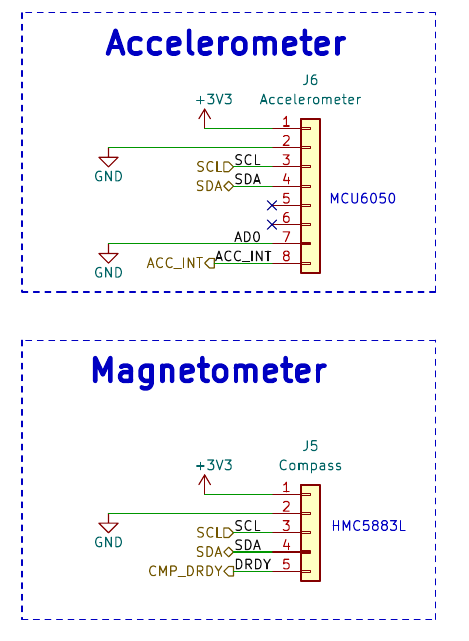
\includegraphics[scale=0.6]{figures/image31.png}
\captionsetup{type=figure}
\captionof{figure}{Connettori Accelerometro e Magnetometro}
\end{center}

\hypertarget{connettore-display-oled}{%
\subsubsection{\texorpdfstring{Connettore display OLED\\
}{Connettore display OLED }}\label{connettore-display-oled}}

Abbiamo previsto un connettore per un display \emph{OLED 128 x 64} con
controller integrato \emph{SSD1306} al fine di presentare all'utente una
immediata visualizzazione dei dati della scheda e del pannello solare.\\
Tuttavia, non avendo avuto a disposizione il componente durante la fase
di assemblaggio, in questa release non è fisicamente presente.

\begin{center}
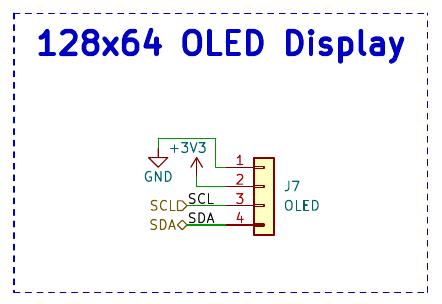
\includegraphics[scale=0.7]{figures/image58.png}
\captionsetup{type=figure}
\captionof{figure}{Connettore display OLED 128x64}
\end{center}

\hypertarget{led-rgb}{%
\subsubsection{\texorpdfstring{\hfill\break
\hfill\break
LED RGB}{  LED RGB}}\label{led-rgb}}

Per quanto riguarda il circuito del led \emph{RGB 1210} abbiamo commesso
un errore in fase di progettazione: considerandone la posizione, tra
collettore ed emettitore del transistor cadranno circa
12-(3.3-0.7)=9.4V!\\
Conseguentemente ai capi dei diodi led cadrà una tensione molto bassa,
probabilmente nemmeno sufficiente per portarli in conduzione.\\
Purtroppo il problema non è sistemabile, se non modificando il circuito
ed il layout della PCB.

Considerando che il componente è del tutto ausiliario abbiamo potuto
testare comunque la scheda senza alcun problema.

\begin{center}
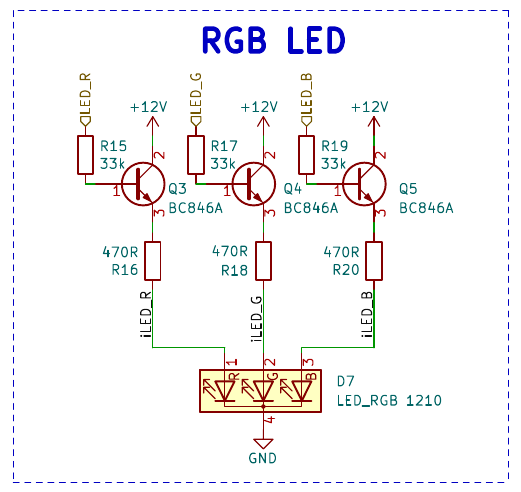
\includegraphics[width=3.68946in,height=3.49479in]{figures/image17.png}
\captionsetup{type=figure}
\captionof{figure}{Circuito led RGB 1210}
\end{center}

\hypertarget{buzzer}{%
\subsubsection{\texorpdfstring{\hfill\break
\hfill\break
Buzzer}{  Buzzer}}\label{buzzer}}

Abbiamo previsto un buzzer passivo di tipo elettromagnetico per poter
segnalare eventuali stati all'utente e/o errori. Per amplificare il
segnale proveniente dall'RP2040 abbiamo utilizzato un transistor NPN con
rete di polarizzazione integrata ed un resistore in parallelo al
cicalino per poter scaricare la tensione imposta dall'induttanza del
buzzer, che altrimenti danneggerebbe il transistor.

\begin{center}
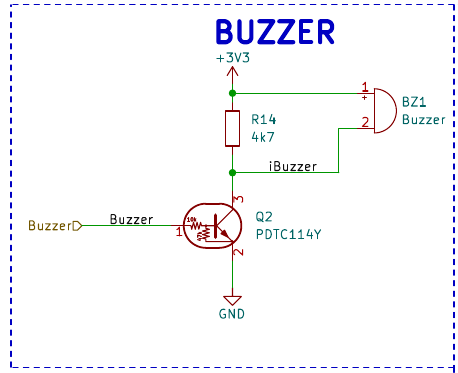
\includegraphics[width=3.08958in,height=2.51619in]{figures/image38.png}
\captionsetup{type=figure}
\captionof{figure}{Circuito buzzer}
\end{center}

\hypertarget{panel-sensing}{%
\section{\texorpdfstring{Panel sensing}{ Panel sensing}}\label{panel-sensing}}

\begin{center}
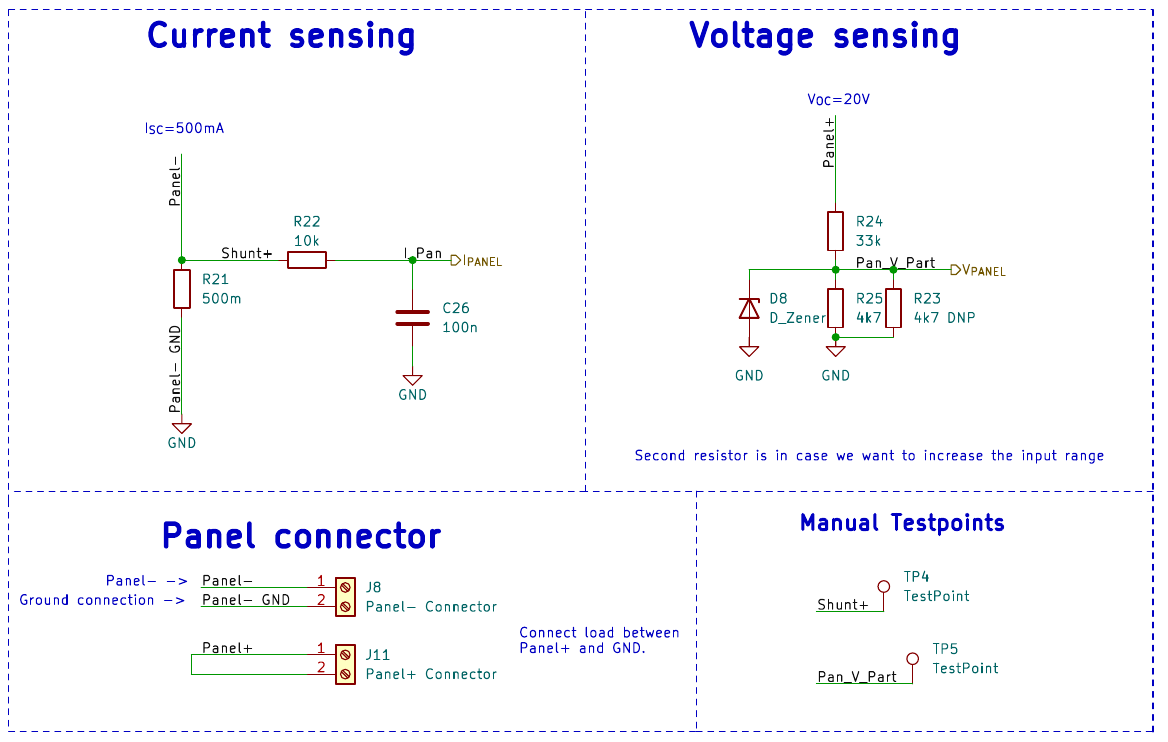
\includegraphics[width=6.5in,height=4.125in]{figures/image24.png}
\captionsetup{type=figure}
\captionof{figure}{Foglio "Panel Sensing" SALMO\newline}
\end{center}

Il panel sensing è stato progettato per la misura dei parametri di
tensione e di corrente del pannello solare. La misura di corrente del
pannello tiene conto di una corrente di cortocircuito (\emph{Isc}) pari
a \emph{500 mA}. Per effettuare la misura è stata posta una resistenza
di shunt pari a 500 mΩ per ottenere una misura di tipo \emph{low-side},
ottenendo così una caduta di tensione ai suoi capi massima di 0.25V che
può essere letta senza problemi dall'ADC dell'RP2040 (GPIO27, canale 2
dell'ADC).\\
Nella scelta della resistenza di shunt, condizionata dal fatto che non
volevamo complicare inutilmente il circuito con degli amplificatori
operazionali, è stato dato maggior peso alla potenza dissipata che allo
sfruttare in maniera ottimale il range dell'ADC.\\
La tensione misurata dall'ADC andrà infatti da 0V (Ipanel=0 A) a 0.25 V
(Ipanel=Isc=500 mA) e la potenza dissipata massima sarà quindi
\(R*I^{2}\  = 0.5*0.5^{2} = 0.125\ W\).\\
Avendo un \emph{ADC} a 12 bit, è possibile ottenere una sensibilità di
\(\frac{(Vref - Vss)}{2^{\text{bit}}} = \frac{3.3}{2^{12}} = 805.66\ uV/bit\)
, corrispondente a
\(\frac{(Vref - Vss)}{2^{\text{bit}}*0.5} = \frac{3.3}{2^{11}} = 1.6\ mA/bit\).
Data la Vmax di segnale pari a 0.25 V è possibile sfruttare solamente il
7.6\% dell'intero range disponibile
(\(\frac{\text{Vref}}{\text{Vmax}} = \frac{3.3}{0.25} = 7.26\%\))

\begin{center}
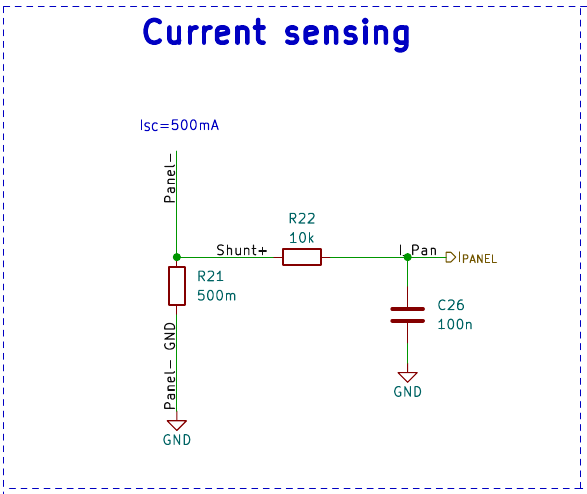
\includegraphics[width=4.19954in,height=3.53646in]{figures/image19.png}
\captionsetup{type=figure}
\captionof{figure}{Circuito Current Sensing SALMO\newline}
\end{center}

Per la misura di tensione del pannello, non volendo nuovamente
utilizzare amplificatori operazionali o integrati specifici, abbiamo
scelto di utilizzare il metodo del partitore di tensione, posizionando
due resistenze da 33k e 47k per avere un rapporto di partizione di circa
\(\frac{4,7}{4,7 + 33} \simeq \ 0.125\). Assumendo di avere un pannello
con tensione di open circuit \emph{Voc} di 20V, i valori in ingresso al
GPIO 26 (canale numero 1 dell'ADC) andranno da 0V a 2.5V (la tensione
massima è comunque fissata dal diodo zener di protezione posto in
parallelo).
\({V_{\text{PANE}{L - MAX}_{\text{ADC}}} = V}_{panel +}*(\frac{R_{25}}{R_{25} + R_{24}}) = 20*0.125\  = 2.5\ V\ \)

Nel caso in cui il pannello avesse tensione di open circuit più alta o
volessimo usare più pannelli in serie tra di loro è possibile montare la
resistenza ausiliaria R23, che permette di avere un rapporto di
partizione di 0.067.

\({V_{\text{PANE}{L - MAX}_{\text{ADC}}} = V}_{panel +}*(\frac{R_{25}}{R_{25} + R_{24}}) = 20*0.067\  = 1.34\ V\)

\begin{center}
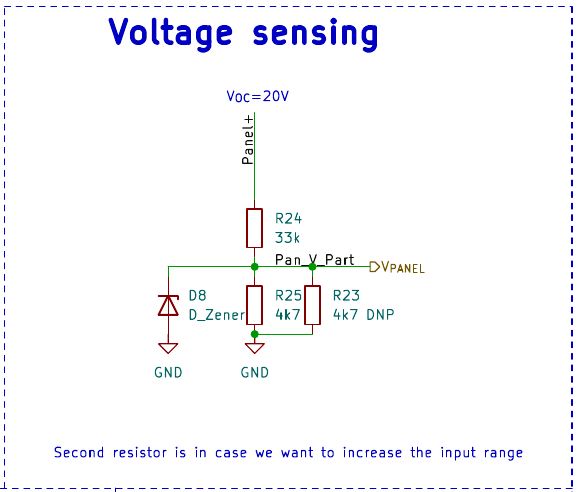
\includegraphics[scale=0.7]{figures/image62.png}
\captionsetup{type=figure}
\captionof{figure}{Circuito Voltage Sensing SALMO\newline}
\end{center}

In questo foglio abbiamo inoltre deciso di posizionare i connettori per
il collegamento del pannello e del relativo carico/utilizzatore.

\begin{center}
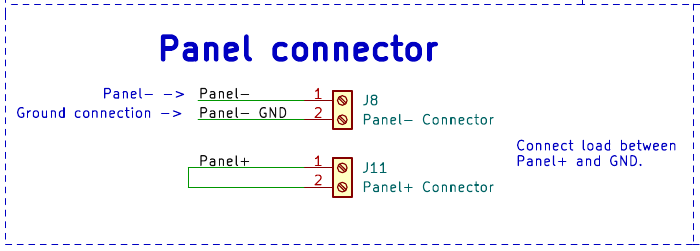
\includegraphics[scale=0.8]{figures/image48.png}
\captionsetup{type=figure}
\captionof{figure}{Connettori per carico e pannello SALMO\newline}
\end{center}

Abbiamo infine inserito dei test point per consentirci di misurare
manualmente la tensione e la corrente del pannello (misurando la caduta
di tensione sulla resistenza di shunt si ottiene
\(i\  = \frac{V_{\text{misurata}}}{R_{21}}\)).

\begin{center}
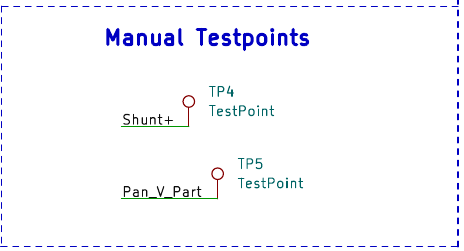
\includegraphics[scale=0.8]{figures/image70.png}
\captionsetup{type=figure}
\captionof{figure}{Testpoint per la misura manuale di tensione e corrente del pannello}
\end{center}

\hypertarget{actuation}{%
\section{Actuation}\label{actuation}}

\begin{center}
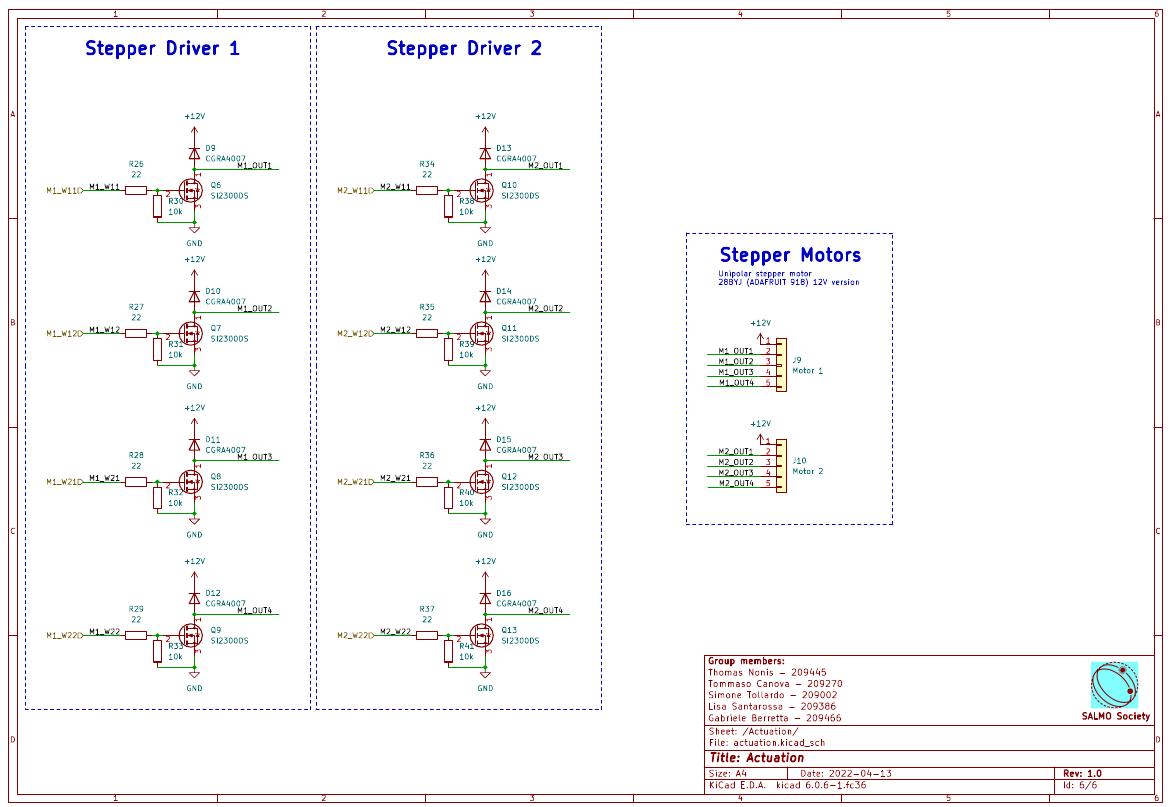
\includegraphics[width=6.5in,height=4.48611in]{figures/image41.png}
\captionsetup{type=figure}
\captionof{figure}{Foglio "Actuation" SALMO\newline}
\end{center}

La pagina dello schematico chiamata \emph{Actuation} prevede il comando
di due motori stepper unipolari tramite driver separati a
componentistica discreta e i relativi connettori. I due attuatori hanno
la funzione di orientare il pannello fotovoltaico nella direzione
desiderata, ruotando il pannello attorno agli assi \emph{z} e \emph{y}.

Abbiamo scelto i motori passo-passo \emph{Adafruit 918}, con tensione e
corrente nominali rispettivamente di 12V e 500mA, unipolari con
motoriduttore e coppia statica di 250gr/cm.

Da evidenziare è la presenza del motoriduttore (\emph{gearbox}) che
permette di ottenere una maggiore risoluzione (da 200 step fino a ben
512) e soprattutto una \emph{maggior coppia statica}; quest'ultima ci
consente di mantenere in posizione il pannello anche quando il motore è
disalimentato così da limitare i consumi totali. Ipotizzando, infatti,
il peso medio di un pannello fotovoltaico da 1W disponibile in commercio
di circa 20gr, una coppia statica di 250gr/cm risulta sufficiente per
consentire di ancorare meccanicamente a dovere il pannello all'asse del
motore.

\hypertarget{section-4}{%
\subsubsection{}\label{section-4}}

Per giunta, ogni motore essendo di tipo unipolare è dotato di due
avvolgimenti separati con presa intermedia comune pertanto sono
sufficienti solo quattro transistor per il comando del singolo. Infatti
a differenza degli stepper bipolari, non è necessario un \emph{h-bridge}
per cambiare il senso di rotazione ma basta invertire l'ordine
sequenziale di attivazione dei transistor. A seguito è illustrato il
circuito base a confronto:

\begin{center}
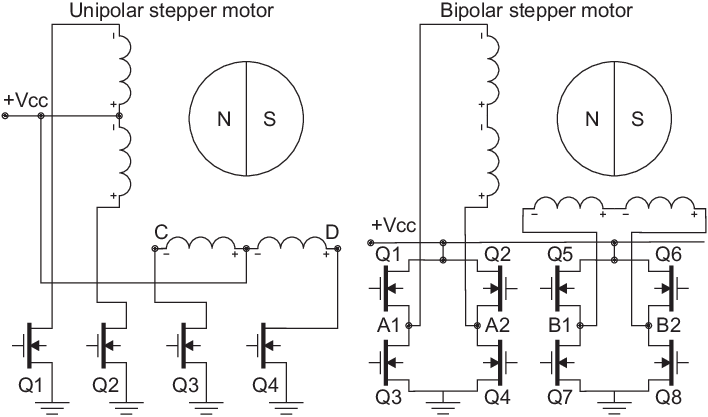
\includegraphics[scale=0.6]{figures/image75.png}
\captionsetup{type=figure}
\captionof{figure}{Driver per stepper unipolare vs driver per stepper bipolare\newline}
\end{center}

Il driver consiste nel porre in serie ad ogni fase del motore un n-mos
pilotato dal MCU, con resistenza di terminazione da 10kΩ e resistenza di
limitazione da 22Ω. La prima funge da pull-down nel caso in cui il pin
del MCU sia flottante, al fine di evitare accensioni involontarie del
transistor, pertanto abbiamo scelto il valore di 10kΩ analogamente alle
altre resistenze di pull-up/down già presenti nel circuito. Invece, la
resistenza da 22Ω limita la corrente sul ramo che connette il pin I/O al
gate del mosfet introducendo un ritardo nel fenomeno di carica e scarica
della capacità di gate-source del dispositivo, evitando così di bruciare
il pin del MCU dato che all'inserzione questa corrente può essere
elevata. Il valore di 22Ω è stato scelto arbitrariamente e fa sì che sul
gate del transistor ci sia una tensione di circa 3.3V (considerando il
partitore tra R26 e R27) quando il pin di output del microcontrollore è
a livello logico alto e, inoltre, determina una costante di
carica/scarica della capacità di ingresso di Q6 di:

\(\backslash tau = R\_\{ 26\}\ \backslash cdot\ C\_\{ gate - source\} = \ 22\backslash Omega\ \backslash cdot\ 7.3nF\ \backslash approx\ 160ns\)\(\)

Una costante di tempo di tale grandezza è considerata accettabile,
perchè ipotizzando una frequenza di lavoro dei mosfet di circa 20Hz,
quindi con un periodo di 55ms, permette allo switch di commuttare come
previsto.

In parallelo alle sezioni di avvolgimenti abbiamo inserito un diodo di
flyback cosicché all'apertura dello switch non si verifichino spike di
tensione critici tra drain e source dello stesso.

\begin{center}
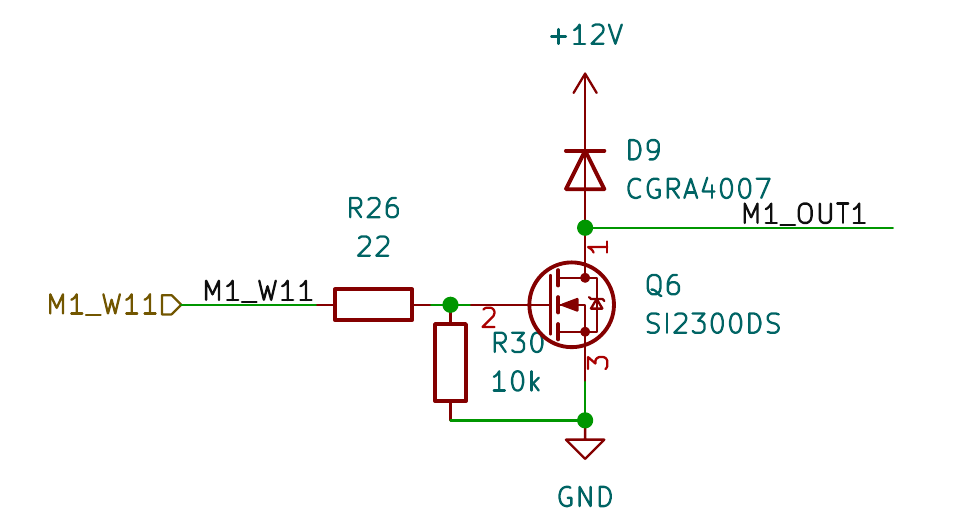
\includegraphics[scale=0.5]{figures/image63.png}
\captionsetup{type=figure}
\captionof{figure}{Circuito driver per un avvolgimento\newline}
\end{center}

Nel circuito in questione lo switch deve garantire:

\begin{enumerate}
\def\labelenumi{\arabic{enumi}.}
\item
  \begin{quote}
  di poter essere pilotato con una tensione di gate di almeno 3.3V
  (livello logico alto dei GPIO del MCU scelto);
  \end{quote}
\item
  \begin{quote}
  una corrente di drain di almeno 0.5A (corrente nominale dei motori);
  \end{quote}
\item
  \begin{quote}
  una differenza di potenziale tra drain e source di almeno 12V
  (tensione di alimentazione dei motori).
  \end{quote}
\end{enumerate}

Considerando le specifiche appena elencate abbiamo scelto dei transistor
Vishay SI2300DS nel comune package SOT23, con tensione di soglia 1.5V e
valori massimi supportati tra drain e source di 30V, tra gate e source
di 12V e una corrente di 3A.

\begin{center}
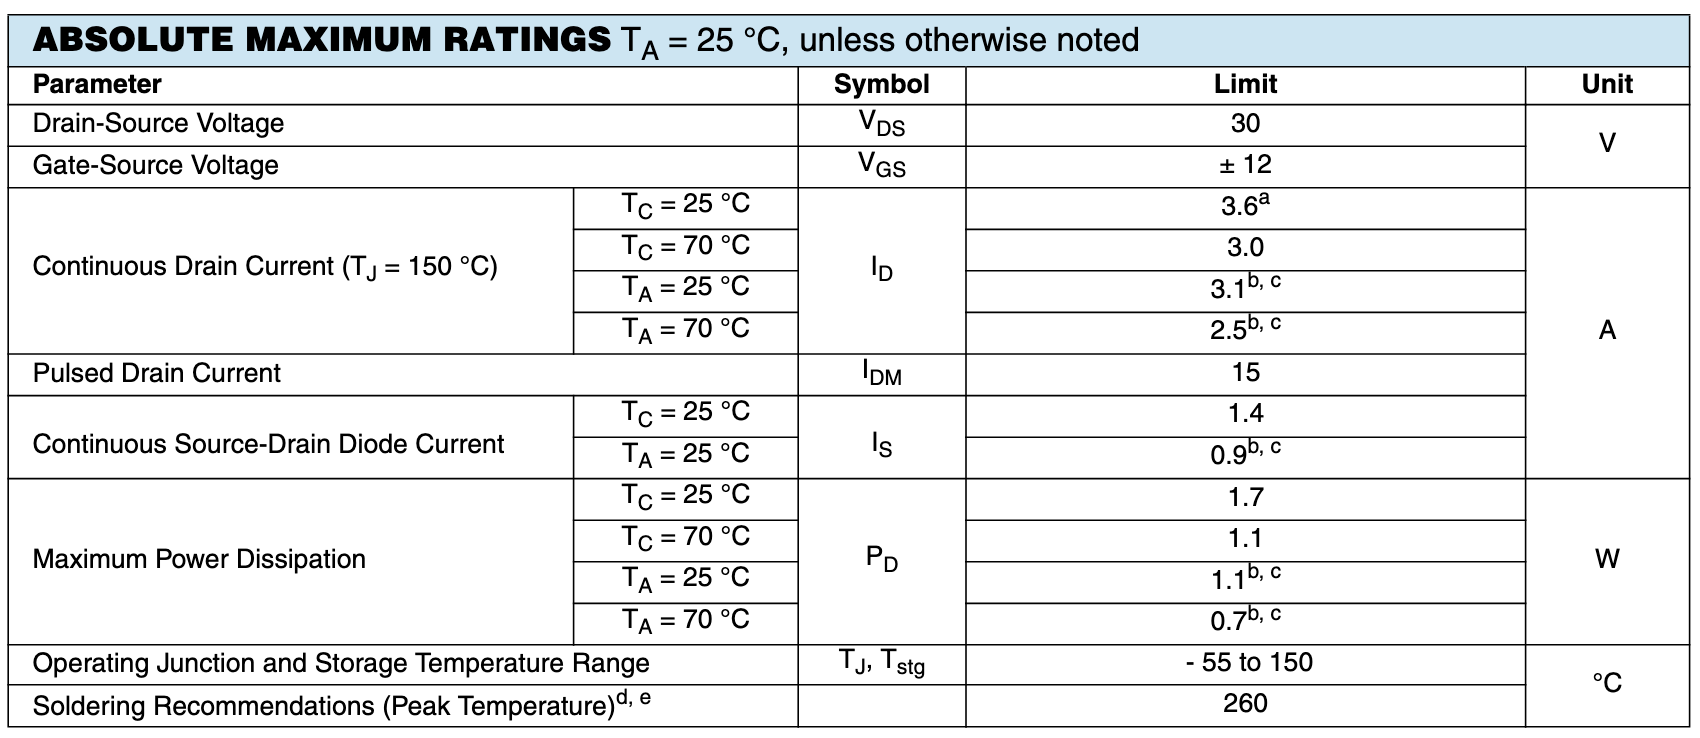
\includegraphics[scale=0.5]{figures/image69.png}
\captionsetup{type=figure}
\captionof{figure}{Estratto datasheet SI2300DS}
\end{center}